\section{Lebesgue: Beyond Slicing to Measuring the Infinite(1902)}


\subsection{The Key Idea: Measuring What Matters}

\textbf{Henri Lebesgue} recognized that \textbf{Émile Borel}’s early attempts at formalizing integration had taken a crucial first step: defining a measure—the mathematical notion of “size”—for sets more general than just intervals. Borel's method allowed mathematicians to assign lengths to sets that were far more fragmented and irregular than anything Riemann had dealt with. But Lebesgue saw that something deeper was needed.

Borel’s construction worked well for simple cases, but it still leaned heavily on the structure of the real number line and on summing over sets in a relatively limited way. It couldn't fully capture the bizarre and pathological behaviors that were now being discovered across analysis—functions that jumped wildly, that were discontinuous everywhere, or that existed only as counterexamples to everything classical calculus held dear.

Lebesgue’s critical insight was that the act of integration wasn’t really about summing along the \( x \)-axis at all. It was about understanding the distribution of a function’s values and how much “space” each of those values occupied. In this view, it didn’t matter whether a function was nice or continuous—what mattered was how often each value occurred, and how large the set was where it occurred.

This shift—from Borel’s set-measure scaffolding to Lebesgue’s full reorientation of the integration process—was a turning point. It made possible a new kind of calculus: one that could handle the modern beasts of analysis, not just the tame functions of the past.

\begin{quote}
Instead of slicing up the domain like Riemann integration, Lebesgue shifted the perspective: \textbf{What if we grouped together points where the function takes the same value and measured those instead?}
\end{quote}

This realization—that some functions were simply too irregular for Riemann’s approach—led to a bold new perspective: what if we flipped the logic of integration entirely?

Rather than slicing the input domain into tiny intervals and summing up the function’s values over them (as Riemann did), the mathematician Henri Lebesgue proposed a radical reversal. He asked: instead of focusing on where the function is defined, why not focus on what values the function takes, and how "big" the sets are that correspond to those values?

In other words, Lebesgue integration doesn’t care so much about the intervals along the x-axis—it measures the size of the sets where the function equals a certain height. Then, it weighs those values accordingly. This shift—from slicing the domain horizontally to slicing the range vertically—gave mathematicians a far more powerful framework.

Suddenly, functions that once defied integration—like the notorious Dirichlet function—could now be measured. The chaos that broke Riemann’s sums could be tamed by Lebesgue’s lens. Where Riemann needed continuity and order, Lebesgue thrived on structure and measure.

Imagine you're watching the graph of a function—not trying to slice it up into tiny rectangles like Riemann would, but instead asking a different question:  

\begin{quote}
\emph{“How much of the $x$-axis lies beneath the parts of the function that are above a certain height?”}
\end{quote}

That’s the heart of the Lebesgue approach.

Rather than chopping the domain into equal-width intervals and summing up the vertical slices (as in Riemann integration), Lebesgue flipped the script. He looked at the \textbf{heights} the function could take, and for each height \( a \), he asked:
\begin{quote}
\emph{“Where is the function greater than this height?”}
\end{quote}

In other words, for each level \( a \), he considered the set of all \( x \)-values where \( f(x) > a \). If you can measure the \textbf{size} of this set (in the sense of length, area, volume, etc.), you can build up the integral by summing across these slices of height.

This reframing gave mathematicians a new superpower: the ability to integrate functions that are wildly more irregular than those Riemann could handle. It’s not the function itself that has to behave nicely—it’s the \textbf{structure of the sets} where it takes certain values.

The only requirement? These level sets must belong to the mathematical structure called a \( \boldsymbol{\sigma} \)-algebra—a formal system for keeping track of which sets are “measurable” and which aren’t. As long as the sets where the function exceeds a given value can be measured this way, the function is fair game for Lebesgue integration.

So in essence:  
Lebesgue didn’t ask \textquotedblleft how high is the function over each slice of the domain?\textquotedblright  
He asked \textquotedblleft how much of the domain is associated with a given height?\textquotedblright  

And that small philosophical shift opened the door to a vast new world of mathematics.

\begin{figure}[H]
\centering
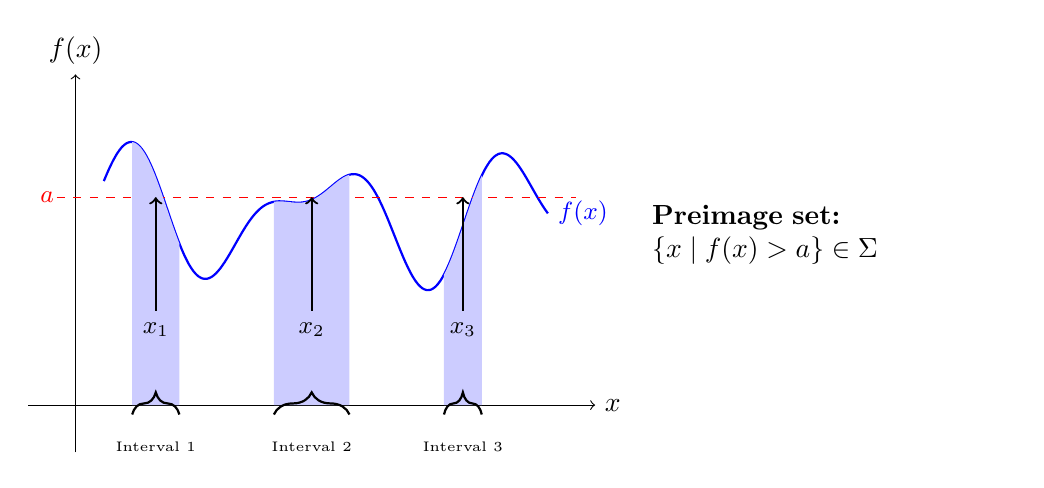
\begin{tikzpicture}[scale=1.2]
    % Axes
    \draw[->] (-0.5,0) -- (5.5,0) node[right] {$x$};
    \draw[->] (0,-0.5) -- (0,3.5) node[above] {$f(x)$};

    % Function curve (irregular)
    \draw[thick, blue, domain=0.3:5, smooth, samples=100] 
        plot (\x, {2 + 0.5*sin(3*\x r) - 0.3*cos(5*\x r)}) node[right] {\small $f(x)$};

    % Horizontal slice at y = a
    \draw[dashed, red] (-0.2,2.2) -- (5.3,2.2);
    \node[red] at (-0.3,2.2) {\small $a$};

    % Highlight the preimage set: where f(x) > a
    \fill[blue!20, domain=0.6:1.1, variable=\x] 
        (0.6,0) -- plot (\x, {2 + 0.5*sin(3*\x r) - 0.3*cos(5*\x r)}) -- (1.1,0) -- cycle;
    \fill[blue!20, domain=2.1:2.9, variable=\x] 
        (2.1,0) -- plot (\x, {2 + 0.5*sin(3*\x r) - 0.3*cos(5*\x r)}) -- (2.9,0) -- cycle;
    \fill[blue!20, domain=3.9:4.3, variable=\x] 
        (3.9,0) -- plot (\x, {2 + 0.5*sin(3*\x r) - 0.3*cos(5*\x r)}) -- (4.3,0) -- cycle;

    % Arrows and labels showing preimages
    \draw[->, thick] (0.85,1) -- (0.85,2.2);
    \draw[->, thick] (2.5,1) -- (2.5,2.2);
    \draw[->, thick] (4.1,1) -- (4.1,2.2);

    \node at (0.85,0.8) {\small $x_1$};
    \node at (2.5,0.8) {\small $x_2$};
    \node at (4.1,0.8) {\small $x_3$};

    % Sigma-algebra label
    \node[align=left, text width=4.5cm, anchor=west] at (6,1.8) {
        \textbf{Preimage set:}\\
        $\{x \mid f(x) > a\} \in \boldsymbol{\Sigma}$
    };

    % Bracket to indicate union of intervals
    \draw[decorate, decoration={brace, amplitude=8pt}, thick]
        (0.6,-0.1) -- (1.1,-0.1) node[midway, below=6pt] {\tiny Interval 1};
    \draw[decorate, decoration={brace, amplitude=8pt}, thick]
        (2.1,-0.1) -- (2.9,-0.1) node[midway, below=6pt] {\tiny Interval 2};
    \draw[decorate, decoration={brace, amplitude=8pt}, thick]
        (3.9,-0.1) -- (4.3,-0.1) node[midway, below=6pt] {\tiny Interval 3};
\end{tikzpicture}
\caption{Instead of slicing the domain (as in Riemann), Lebesgue integration slices the range and looks at the measure of preimage sets where \( f(x) > a \). These sets must belong to the sigma-algebra \( \boldsymbol{\Sigma} \) of measurable sets.}
\end{figure}


This figure visually demonstrates the foundational idea of Lebesgue integration: instead of slicing the domain into small intervals (as in Riemann integration), we fix a horizontal level \( a \) in the codomain (range), and then examine the \emph{preimage} of this level—i.e., the set of \( x \)-values where the function \( f(x) \) lies above that level. These horizontal "slices" of the range carve out subsets of the domain, shown here as shaded intervals. The key requirement is that these subsets must belong to the sigma-algebra \( \boldsymbol{\Sigma} \) of measurable sets. By systematically scanning through all values of \( a \), we accumulate the contributions of the function over these measurable regions. This method allows the Lebesgue integral to handle more irregular and discontinuous functions than the Riemann approach, since it depends on how much of the domain lies within certain vertical thresholds, rather than how the function behaves within each domain slice. In essence, it measures the "size" of the set of inputs for which the function exceeds a given value, and integrates over that.



\subsection{From Range to Measure: Visualizing the Logic of Lebesgue Integration}

\textbf{Overview.} These four figures tell the story of Lebesgue integration by shifting our perspective from slicing the domain (as in Riemann) to slicing the \emph{range} of the function.

\begin{figure}[H]
\centering
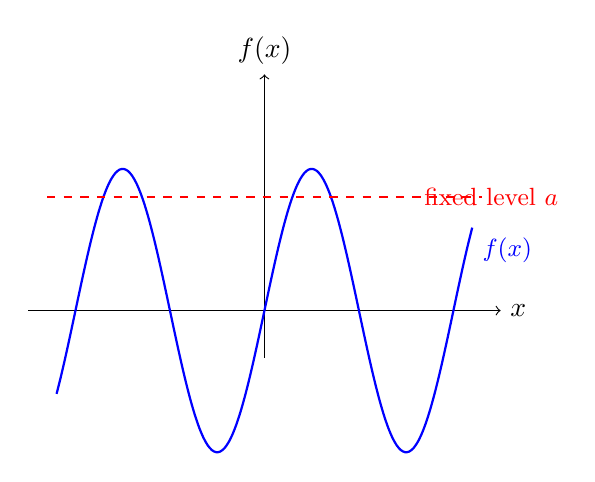
\begin{tikzpicture}[scale=1.2]
    % Function plot
    \draw[->] (-2.5,0) -- (2.5,0) node[right] {$x$};
    \draw[->] (0,-0.5) -- (0,2.5) node[above] {$f(x)$};

    \draw[thick, blue, domain=-2.2:2.2, samples=100, smooth] plot (\x, {1.5*sin(180*\x)}) node[below right] {\small $f(x)$};

    % Horizontal line at y = a
    \draw[dashed, red, thick] (-2.3,1.2) -- (2.3,1.2);
    \node[red] at (2.4,1.2) {\small fixed level $a$};
\end{tikzpicture}
\caption{Instead of dividing the domain into small intervals like Riemann integration, we begin by fixing a horizontal level $a$ in the range.}
\end{figure}

\begin{figure}[H]
\centering
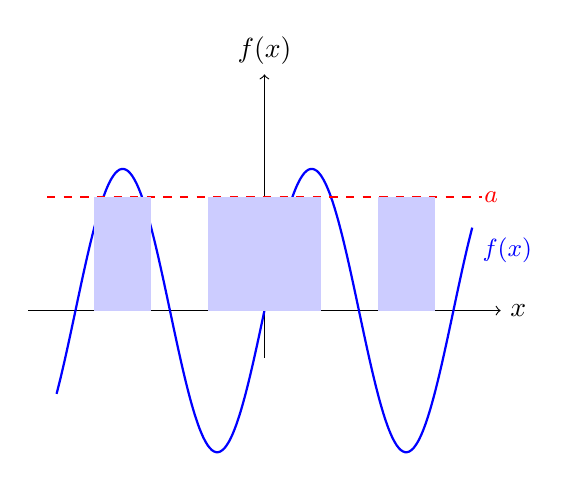
\begin{tikzpicture}[scale=1.2]
    % Axes
    \draw[->] (-2.5,0) -- (2.5,0) node[right] {$x$};
    \draw[->] (0,-0.5) -- (0,2.5) node[above] {$f(x)$};

    % Function
    \draw[thick, blue, domain=-2.2:2.2, samples=100, smooth] plot (\x, {1.5*sin(180*\x)}) node[below right] {\small $f(x)$};

    % Horizontal level a
    \draw[dashed, red, thick] (-2.3,1.2) -- (2.3,1.2);
    \node[red] at (2.4,1.2) {\small $a$};

    % Shaded preimage regions
    \fill[blue!20] (-1.8,0) rectangle (-1.2,1.2);
    \fill[blue!20] (-0.6,0) rectangle (0.6,1.2);
    \fill[blue!20] (1.2,0) rectangle (1.8,1.2);
\end{tikzpicture}
\caption{We then examine the preimage: the set of $x$-values where $f(x) > a$. These regions represent where the function lies above the threshold.}
\end{figure}

\begin{figure}[H]
\centering
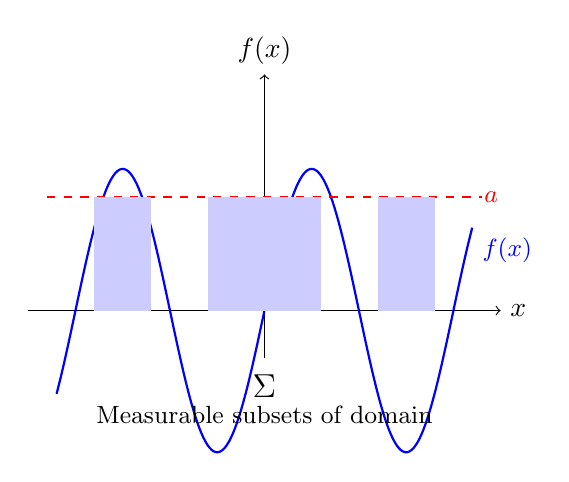
\begin{tikzpicture}[scale=1.2]
    \draw[->] (-2.5,0) -- (2.5,0) node[right] {$x$};
    \draw[->] (0,-0.5) -- (0,2.5) node[above] {$f(x)$};

    \draw[thick, blue, domain=-2.2:2.2, samples=100, smooth] plot (\x, {1.5*sin(180*\x)}) node[below right] {\small $f(x)$};

    \draw[dashed, red, thick] (-2.3,1.2) -- (2.3,1.2);
    \node[red] at (2.4,1.2) {\small $a$};

    \fill[blue!20] (-1.8,0) rectangle (-1.2,1.2);
    \fill[blue!20] (-0.6,0) rectangle (0.6,1.2);
    \fill[blue!20] (1.2,0) rectangle (1.8,1.2);

    % Sigma symbol and measurable set label
    \node at (0,-0.8) {\large$\boldsymbol{\Sigma}$};
    \node at (0,-1.1) {\small Measurable subsets of domain};
\end{tikzpicture}
\caption{Each of these $x$-intervals forms a subset of the domain. For $f$ to be Lebesgue measurable, these sets must belong to the $\boldsymbol{\Sigma}$-algebra of measurable sets.}
\end{figure}

\begin{figure}[H]
\centering
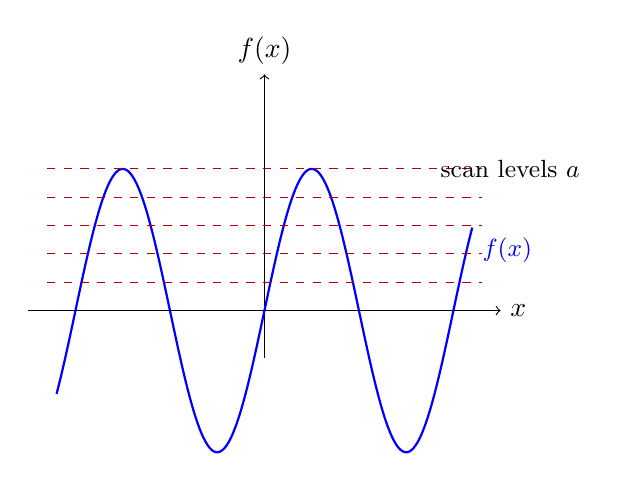
\begin{tikzpicture}[scale=1.2]
    \draw[->] (-2.5,0) -- (2.5,0) node[right] {$x$};
    \draw[->] (0,-0.5) -- (0,2.5) node[above] {$f(x)$};

    \draw[thick, blue, domain=-2.2:2.2, samples=100, smooth] plot (\x, {1.5*sin(180*\x)}) node[below right] {\small $f(x)$};

    % Several horizontal levels
    \foreach \y in {0.3, 0.6, 0.9, 1.2, 1.5} {
        \draw[dashed, red!70!black] (-2.3,\y) -- (2.3,\y);
    }

    \node at (2.6,1.5) {\small scan levels $a$};
\end{tikzpicture}
\caption{By scanning all horizontal levels $a$, we integrate how much of the domain lies above each threshold. This defines the Lebesgue integral.}
\end{figure}

\vspace{1em}
\noindent
\textbf{Conclusion.} Lebesgue integration tells a different story than Riemann: rather than summing rectangles over small domain intervals, we measure the total "size" of inputs that exceed each function value. This strategy handles more functions, more irregularities, and more real-world behavior—especially when data is messy or fragmented.





\subsection{Generalizing Integration: Integrating Over Measurable Sets}

Traditional Riemann integration works by partitioning an \textbf{interval} into smaller subintervals and summing function values over them. However, this approach struggles with pathological functions, where intervals fail to provide a meaningful structure.

Lebesgue's insight was to generalize integration beyond intervals. Instead of integrating over a fixed interval, he proposed integrating over measurable sets, which are sets that can be assigned a measure equivalent to an interval.

\begin{quote}
\textbf{If a set can be mapped to an interval in a meaningful way, then we can define an integral over it.}
\end{quote}

This concept sounds simple in theory but is incredibly difficult in practice:

\begin{itemize}
    \item Finding the right measure is non-trivial. While Lebesgue measure works well in \(\mathbb{R}\), other spaces require different measures (e.g., Haar measure in group theory, probability measures in statistics).
    \item Not all sets are measurable. Some sets, like those constructed using the Axiom of Choice (e.g., the Vitali set), resist any meaningful notion of measure.
    \item Automating this process is impractical. While computers can compute Riemann integrals symbolically or numerically, determining the correct measure for a given problem often requires deep mathematical insight and domain-specific knowledge.
\end{itemize}

Thus, while Lebesgue integration vastly expands what can be integrated, it does so at the cost of requiring a much deeper understanding of the structure of the set over which the function is being integrated.

\subsection{Why This Was Revolutionary}

Lebesgue’s insight resolved the fundamental issue with Borel’s method. By focusing on measuring values instead of partitioning the domain, he created a framework that could integrate even wildly discontinuous functions.

Unlike the Riemann integral, which sums function values over small partitions, the Lebesgue integral sums over values of the function itself, grouping points that share the same function value and measuring their total "size" in the domain. 

If these level sets are measurable, the function can be integrated via the Lebesgue integral:

\[
\int f \, d\mu = \int_0^\infty \mu(\{ x \mid f(x) > a \}) \, da.
\]

If these level sets are not measurable—like in the case of the Dirichlet function (which is 1 on rationals and 0 on irrationals)—then the function cannot be properly integrated in the Lebesgue sense.

Lebesgue’s generalization of integration to measurable sets fundamentally reshaped modern analysis. By removing the dependency on rigid intervals, he expanded integration to work in settings that Riemann’s approach never could, paving the way for applications in functional analysis, probability theory, and even modern physics.

\subsection{Why the Dirichlet Function's Integral is Zero}

\subsubsection{When Zero Means Everything: Lebesgue Measure and the Vanishing Rationals}

In measure theory, we now recognize a crucial fact:

\begin{itemize}
    \item The set of \textbf{rational numbers} \( \mathbb{Q} \) is \textbf{countable} and therefore has \textbf{Lebesgue measure zero}.
    \item The set of \textbf{irrational numbers} \( \mathbb{R} \setminus \mathbb{Q} \) is \textbf{uncountable} and has \textbf{full measure}.
\end{itemize}

This means that, under Lebesgue integration, the contribution of the rationals to the integral is entirely **insignificant**—no matter how many rational numbers exist, their **total measure is still zero**.

Thus, when computing the Lebesgue integral of the Dirichlet function over any interval \( [a, b] \):

\[
\int_a^b D(x) \,dx = \int_a^b 1 \cdot \mathbb{1}_{\mathbb{Q}}(x) \,dx,
\]

where \( \mathbb{1}_{\mathbb{Q}}(x) \) is the indicator function of the rationals, we find that:

\[
\int_a^b D(x) \,dx = 0.
\]

This is because the integral assigns weight (measure) to sets, and the rationals are simply **too small** to contribute anything measurable.

\subsubsection{An Intuitive Analogy: How Fourier’s Microphone Silences the Dirichlet Function}

Imagine you’re at a massive concert venue, and your job is to measure the overall loudness of the crowd.

\begin{itemize}
    \item Rational numbers (1s) are the people who occasionally cheer—random bursts of noise scattered throughout the audience.
    \item Irrational numbers (0s) are the people who just sit there in total silence.
\end{itemize}

Now, you pull out a fancy microphone designed to record the average volume of the entire stadium. But when you listen back to the recording…  

\textbf{Silence. Nothing. Zero.}  

Why? Because while the cheerers do exist, they’re spread so thin that their total contribution is mathematically insignificant. The silent majority (the irrationals) dominates, and the final measurement tells you the entire stadium was dead quiet—even though, if you were standing in the middle of the crowd, you’d hear sporadic cheering all around you.  

This is exactly what happens with the \textbf{Dirichlet function} in Fourier analysis. The function clearly exists—it takes values of 1 on rational numbers—but when you try to sum up its Fourier coefficients, the contribution from the rationals is completely erased by the sheer overwhelming presence of the irrationals. The final answer?  

\[
f_{\text{Dirichlet}}(x) = 0
\]

At the heart of this phenomenon is a fundamental difference in the sizes of infinities:

\begin{itemize}
    \item The set of \textbf{rational numbers} (\(\mathbb{Q}\)) is \textbf{countable}, meaning it can be listed in a sequence \( q_1, q_2, q_3, \dots \).
    \item The set of \textbf{irrational numbers} (\(\mathbb{R} \setminus \mathbb{Q}\)) is \textbf{uncountable}, meaning its infinity is vastly larger in size.
\end{itemize}

This distinction matters when computing the Fourier coefficients of the Dirichlet function, which involves integrating over an interval. The problem is that a Riemann integral relies on dividing the interval into small subintervals and summing function values at selected points. But here’s the issue:

\begin{quote}
No matter how the subintervals are chosen, every interval will contain both rationals and irrationals. The irrationals dominate in every subinterval, and since the function is zero at all irrationals, the contribution from the rationals is effectively lost.
\end{quote}

Unlike functions that behave smoothly or have well-defined jumps, the Dirichlet function is erratic everywhere—jumping between 0 and 1 infinitely often in any interval. This makes it impossible for the Riemann sum to converge to anything meaningful. Since the irrationals are vastly more numerous than the rationals, the integral ultimately evaluates to zero, meaning the Fourier coefficients vanish.

To return to the concert analogy: even if the rational numbers (cheering people) are \textbf{densely packed} throughout the stadium, their total contribution is mathematically insignificant compared to the overwhelming silence of the irrationals.

Thus,  

\begin{quote}
\textbf{An uncountable amount of silence drowns out a countable amount of noise, leaving nothing behind.}  
\end{quote}

Fourier’s method, like the microphone, is designed to capture the overall structure of a function, but when applied to the Dirichlet function, it hears only silence.



\subsubsection{Why Lebesgue’s Approach is the Right One}

The failure of the Dirichlet function to be meaningfully integrated under Riemann’s framework was an early indication that a deeper approach was needed. With Lebesgue’s method, we see why this function is problematic **not because it lacks structure, but because its structure is measure-theoretically insignificant**.

By shifting the focus from partitioning intervals to measuring function values, Lebesgue **solved a century-old problem** and created a foundation for modern analysis. And in doing so, he finally answered the question that Fourier's work had hinted at:

\begin{quote}
\textbf{Some functions are just too "thin" to make an impact. And when you try to integrate them, they vanish into mathematical silence.}
\end{quote}


\subsection{Beyond Silence: Who Decides What’s Measurable?}

\subsubsection{The Measurability Debate: Intuition vs. Abstraction}

By the time Lebesgue formalized his approach to integration, it was clear that measure theory had reshaped our understanding of what functions could be tamed—and which would vanish into noise. But behind the mathematics was a deeper debate: \textbf{how far should we go in defining measurable sets?}

On one side were those who valued concreteness and intuition—mathematicians who believed that only explicitly constructible sets deserved to be studied. On the other were those who embraced abstraction, willing to work with sets that couldn’t even be visualized or written down explicitly.

This wasn’t just a technical disagreement—it was a philosophical rift about the foundations of mathematics itself.

And at the heart of this divide stood two towering figures: \textbf{Émile Borel} and \textbf{Henri Lebesgue}.

\subsubsection{Borel’s Approach: Keep Things Constructive and Intuitive}

Émile Borel was a pioneer in probability theory and one of the first to formalize the idea of measure. However, he had a more \textbf{pragmatic} and \textbf{constructivist} view of mathematics:

\begin{itemize}
    \item He believed that mathematics should be based on \textbf{explicit constructions}, not just abstract existence proofs.
    \item He was skeptical of \textbf{highly pathological sets}, particularly those arising from Cantor’s set theory.
    \item Borel’s measure theory was limited to \textbf{Borel sets}—the smallest class of sets generated from open intervals through countable unions, intersections, and complements.
\end{itemize}

\subsubsection{Lebesgue’s Expansion: The Need for a More General Theory}

Lebesgue, on the other hand, wanted to \textbf{expand measure theory beyond Borel’s framework}. He recognized that in order to make integration truly universal, one had to measure sets that were even more irregular than Borel’s.

\begin{itemize}
    \item He was willing to work with more \textbf{abstract and general objects}, even if they lacked constructive definitions.
    \item He extended the concept of measurability beyond Borel sets to a larger class known as \textbf{Lebesgue measurable sets}.
    \item He showed that Borel’s system, while powerful, was \textbf{not enough} to handle all reasonable functions in analysis.
\end{itemize}

\subsubsection{The Core Disagreement: The Role of Pathological Sets}

Borel was deeply uncomfortable with some of the \textbf{non-constructive} sets that Lebesgue allowed in his theory. To Borel, these sets were a mathematical curiosity at best and a dangerous abstraction at worst.

\begin{quote}
\textbf{“Mathematics should remain connected to reality.”} — Émile Borel
\end{quote}

Lebesgue, however, argued that avoiding these sets would unnecessarily \textbf{restrict} the power of measure theory and integration.

\begin{quote}
\textbf{“Mathematics should be free to explore any logical consequences, no matter how unintuitive they may seem.”} — Henri Lebesgue
\end{quote}




